\documentclass{article}
\usepackage{graphicx} % Required for inserting images

\title{Assignment 3 - Part 1}
\author{Xinyu Meng netid:xm73 RUID:193002567 
\\Qichao Lin netid:ql180 RUID:196005340}
\date{April 2023}
\usepackage{tikz} 
\begin{document}

\maketitle

\section{Problem 1}

Problem 1 (15 points): Consider the following Bayesian network, where variables A through E are all Boolean valued. Note: there is a typo in the image, it should be P(A = true) = 0.2 instead of P(D = true) = 0.2 .

\subsection{a)}
a) What is the probability that all five of these Boolean variables are simultaneously true?

$P(A,B,C,D,E) = P(A)P(B)P(C)P(D\mid A,B)P(E\mid B,C) = 0.2*0.5*0.8*0.1*0.3 = 0.0024$

\subsection{b)}
b) What is the probability that all five of these Boolean variables are simultaneously false? [Hint:Answ(1e5rpsoimintisla)rlytoabove.]

$P(\neg A,\neg B,\neg C,\neg D,\neg E) = P(\neg A)P(\neg B)P(\neg C)P(\neg D\mid \neg A,\neg B)P(\neg E\mid \neg B,\neg C) = 0.8*0.5*0.2*0.1*0.8 = 0.0064$

\subsection{c)}
c) What is the probability that A is false given that the four other variables are all known to be true?

$P(\neg A \mid B, C, D, E) = P(B,C,D,E \mid \neg A)P(\neg A)\div P(B,C,D,E)$
\\
\\based on product rule, we know that $P(B,C,D,E \mid \neg A)P(\neg A) = P(B,C,D,E, \neg A) = P(\neg A)P(B)P(C)P(D\mid \neg A,B)P(E\mid B,C) = 0.8*0.5*0.8*0.6*0.3 = 0.0576$
\\
\\and $P(B,C,D,E) = P(B,C,D,E,A) + P(B,C,D,E,\neg A) = 0.0024 + P(\neg A)P(B)P(C)P(D\mid \neg A,B)P(E\mid B,C) = 0.0024 + 0.8*0.5*0.8*0.6*0.3 = 0.06$
\\
\\Therefore, 
$P(\neg A \mid B, C, D, E) = P(B,C,D,E \mid \neg A)P(\neg A)\div P(B,C,D,E)= 
P(B,C,D,E, \neg A) \div (P(B,C,D,E,A) + P(B,C,D,E,\neg A)) = 0.0576 \div 0.06 = 0.96$


\section{Problem 2}
\subsection{a)}
a) Calculate P(Burglary| JohnsCalls = true, MaryCalls = true) and show in detail the calculations that take place. Use your book to confirm that your answer is correct.

$P(Burglary\mid JohnsCalls = true,MaryCalls = true)
= \alpha P(Burglary, JohnsCalls = true,MaryCalls = true) 
\\= \alpha \sum_{Earthquake}  \sum_{Alarm} P(Burglary, JohnsCalls,MaryCalls,Earthquake, Alarm)
\\= \alpha \sum_{Earthquake}  \sum_{Alarm} P(Burglary) P(JohnsCalls \mid Alarm)P(MaryCalls\mid Alarm)P(Earthquake)P(Alarm\mid Burglary, Earthquake)
\\= \alpha P(Burglary) \sum_{Earthquake} P(Earthquake) \sum_{Alarm}  P(JohnsCalls \mid Alarm)P(MaryCalls\mid Alarm)P(Alarm\mid Burglary, Earthquake)
\\
= \alpha <P(Burglary)*((0.02*(0.9*0.7*0.95+0.05*0.01*0.05))+(0.98*(0.9*0.7*0.94+0.05*0.01*0.06))),P(\neg Burglary)*((0.02*(0.9*0.7*0.95+0.05*0.01*0.05))+(0.98*(0.9*0.7*0.94+0.05*0.01*0.06)))>
= \alpha <0.001*((0.002*(0.9*0.7*0.95+0.05*0.01*0.05))+(0.998*(0.9*0.7*0.94+0.05*0.01*0.06))),0.999*((0.002*(0.9*0.7*0.29+0.05*0.01*0.71))+(0.998*(0.9*0.7*0.001+0.05*0.01*0.999)))>
\\
= \alpha <0.00059224,0.0014919> \approx <0.28416517124,0.71583482875>
$

\subsection{b)}
b) Suppose a Bayesian network has the form of a chain: a sequence of Boolean variables X1,...Xn where Parents(Xi) = {Xi-1} for i = 2,...,n. What is the complexity of computing P(X1|Xn = true) using enumeration? What is the complexity with variable elimination?

For enumeration inference, $P(X_{1}|X_{n}=true) = \alpha \sum_{x_{2}} \sum_{x_{3}}....\sum_{x_{n-1}}P(X1,X2,...,Xn)$,which will be $P(X_{1}|X_{n}=true) = \alpha \sum_{x_{2}} \sum_{x_{3}}....\sum_{x_{n-1}}P(X_{1})P(X_{2} \mid X_{1})...,P(X_{n} \mid X_{n-1})$ there are X1 .... Xn variables, Each of the sums over the values of the variables has 2 terms, so the total number of terms to be multiplied is $2^{n-2}.$ Therefore, the time complexity of computing $P(X1 \mid Xn = true)$ using enumeration is $O(2^{n-2})$

For variable elimination and a singly connected bayesian network with a chain, the complexity for variable elimination is linear therefore, O(n) as the chain structure allows for the computation happen once for each variable. 

\section{Problem 3}
\subsection{a)}
Problem3(20points):
\ When the card holder is travelling abroad, fraudulent transactions are more likely since tourists are prime targets for thieves. More precisely, 1\% of transactions are fraudulent when the card holder is travelling, where as only 0.4\% of the transactions are fraudulent when she is not travelling. On average, 5\% of all transactions happen while the card holder is travelling. If a transaction is fraudulent, then the likelihood of a foreign purchase increases, unless the card holder happens to be travelling. More precisely, when the card holder is not travelling, 10\% of the fraudulent transactions are foreign purchases where as only 1\% of the legitimate transactions are foreign purchases. On the other hand, when the card holder is travelling, then 90\% of the transactions are foreign purchases regardless of the legitimacy of the transactions.

\ Purchases made over the internet are more likely to be fraudulent. This is especially true for card holders who don’t own any computer. Currently, 75\% of the population owns a computer or smart phone and for those card holders, 1\% of their legitimate transactions are done over the internet, however this percentage increases to 2\% for fraudulent transactions. For those who don’t own any computer or smart phone, a mere 0.1\% of their legitimate transactions is done over the internet, but that number increases to 1.1\% for fraudulent transactions. Unfortunately, the credit card company doesn’t know whether a card holder owns a computer or smart phone, however it can usually guess by verifying whether any of the recent transactions involve the purchase of computer related accessories. In any given week, 10\% of those who own a computer or smart phone purchase (with their credit card) at least one computer related item as opposed to just 0.1\% of those who don’t own any computer or smart phone.

\ a) Construct a Bayes Network to identify fraudulent transactions.
What to hand in: Show the graph defining the network and the Conditional Probability Tables associated with each node in the graph. This network should encode the information stated above. Your network should contain exactly six nodes, corresponding to the following binary random variables:
OC : card holder owns a computer or smart phone.
Fraud : current transaction is fraudulent.
Trav : card holder is currently travelling.
FP : current transaction is a foreign purchase.
IP : current purchase is an internet purchase.
CRP : a computer related purchase was made in the past week.
The arcs defining your Network should accurately capture the probabilistic dependencies between these variables.

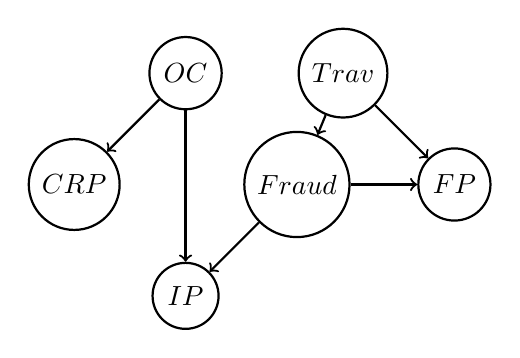
\begin{tikzpicture}[node distance={20mm}, thick,main/.style = {draw, circle}] 
\node[main] (1) {$OC$}; 
\node[main] (2) [below left of=1] {$CRP$};
\draw[->] (1) -- (2);

\node[main] (3) [right of=1]{$Trav$};
\node[main] (4) [below right of=1]{$Fraud$};

\draw[->] (3) -- (4);

\node[main] (5) [right of=4]{$FP$};
\draw[->] (3) -- (5);
\draw[->] (4) -- (5);

\node[main] (6) [below right of=2] {$IP$};
\draw[->] (1) -- (6);
\draw[->] (4) -- (6);


\end{tikzpicture} 


\begin{center}
\begin{tabular}{ |c|c| } 
 \hline
 OC &  $0.75$ \\ 
 $\neg OC$ & $0.25$ \\
 \hline
\end{tabular}
\end{center}

\begin{center}
\begin{tabular}{ |c|c| } 
 \hline
 Transaction during Trav  \\ 
  $0.05$ \\
  
 \hline
\end{tabular}
\end{center}

\begin{center}
\begin{tabular}{ |c|c|c| } 
 \hline
 OC & P(CRP)  \\ 
 True & $0.1$ \\
 False & $0.001$ \\
 \hline
\end{tabular}
\end{center}

\begin{center}
\begin{tabular}{ |c|c|c| } 
 \hline
 Trav & P(Fraud)  \\ 
 True & $0.01$ \\
 False & $0.004$ \\
 \hline
\end{tabular}
\end{center}


\begin{center}
\begin{tabular}{ |c|c|c|c| } 
 \hline
 OC &  Fraud &  P(IP) \\ 
 True & True & 0.02\\
 True & False & 0.01\\
False & True & 0.011\\
 False & False & 0.001\\
 \hline
\end{tabular}
\end{center}

\begin{center}
\begin{tabular}{ |c|c|c|c| } 
 \hline
Fraud & Trav & P(FP)  \\ 
 True & True & $0.9$\\
 False & True & $0.9$\\
 True & False & $0.1$\\
 False & False & $0.01$\\
 \hline
\end{tabular}
\end{center}


b) What is the prior probability (i.e., before we search for previous computer related purchases and before we verify whether it is a foreign and/or an internet purchase) that the current transaction is a fraud? What is the probability that the current transaction is a fraud once we have verified that it is a foreign transaction, but not an internet purchase and that the card holder purchased computer related accessories in the past week?
What to hand in: Indicate the two queries (i.e., P r(variables|evidence)) you used to compute those two probabil- ities. Show each step of the calculation

For the probability of a transaction being fraud, 
$P(Fraud) = P(Fraud\mid Trav) * P(Trav) + P(Fraud\mid \neg Trav) * P(\neg Trav) = 0.01 * 0.05 + 0.004 * 0.95 = 0.0043$

$P(Fraud \mid FP, \neg IP, CRP)$
\
= $\alpha P(Fraud, FP, \neg IP, CRP) $
\\= $\alpha \sum_{Trav} \sum_{OC}P(Fraud, FP, \neg IP, CRP, Trav, OC)$
\\= $\alpha \sum_{Trav} \sum_{OC}P(Fraud\mid Trav)P(FP\mid Trav,Fraud)P(\neg IP\mid OC,Fraud)P(CRP\mid OC)P(Trav)P(OC)$
\\= $\alpha \sum_{Trav}P(Trav)\sum_{OC}P(OC)P(Fraud\mid Trav)P(FP\mid Trav,Fraud)P(\neg IP\mid OC,Fraud)P(CRP\mid OC)$
\\= $\alpha <0.00006121,0.0040239>$
\\ $ \approx <0.0149837,0.9850163>$

Therefore, $P(Fraud \mid FP, \neg IP, CRP) = 0.0149837$

\end{document}
